The back-end readout card for the system under development, the Zynq UltraScale+ RFSoC ZCU216 Evaluation Card, has been chosen taking into consideration the points described in \autoref{sec:selection}.
In this section, the overall architecture and features of the card are presented.
A possibility for evaluation of the card is also demonstrated.
At last, a design for the read-out firmware is proposed and an overview of the firmware elements is given. 

\section{Xilinx ZCU216 Evaluation Card}
The ZCU216 Evaluation Card is equipped with the ZU49DR Zynq Ultrascale+ \gls{rfsoc} (Gen 3). 
It allows for quick evaluation of the on-chip \gls{rf} data converters and quick prototyping of different user-defined systems.

The features which are important for the designed read-out system are listed in the following (as seen in \cite{zcu216}):
\begin{itemize}[noitemsep]
	\item Sixteen 14-bit, \SI{2.5}{\giga \sample \per \second} \gls{rf}-\gls{adc}
	\item Sixteen 14-bit, \SI{10}{\giga \sample \per \second} \gls{rf}-\gls{dac}
	\item I/O expansion options: \gls{fpga} Mezzanine Card (\gls{fmc}+) interfaces, RFMC 2.0 interfaces, and Pmod (peripheral module) connections
	\item \gls{ddr4} \gls{dimm} -- 4 GB, 64-bit, 2.666 MT/s, attached to the \gls{pl}
	\item \gls{ddr4} \gls{sodimm} -- 4 GB, 64-bit, 2.400 MT/s, attached to the \gls{ps}
	\item High-speed I/Os: $2\times2$ \gls{sfp}/SFP+/zSFP+/SFP28 modules
	\item Breakout cards for evaluation of the \gls{adc} and \gls{dac} performance, together with a clock add-on card for internal/external reference clocking
\end{itemize}
Other peripheral connections and features are shown in the top view of the board in \autoref{fig:zcu216}. 

%todo this is a workaround because strangely it doesn't work with includegraphics....
\begin{figure}[tb]
\resizebox{1\textwidth}{!}{
	\begin{tikzpicture}[scale = 1.1]
		\node {\includegraphics[width=8cm]{chap/05-readout/img/zcu216cleared}};
		%left
		\node[fill=none,font=\tiny,align=right,anchor=east] at (-2.1,1.6) {USB (JTAG/UART)};
		\node[fill=none,font=\tiny,align=right,anchor=east] at (-2.1,1.38) {JTAG PC4};
		\node[fill=none,font=\tiny,align=right,anchor=east] at (-2.1,1.13) {Micro SD};
		\node[fill=none,font=\tiny,align=right,anchor=east] at (-2.1,0.9) {Ethernet};
		\node[fill=none,font=\tiny,align=right,anchor=east] at (-2.1,0.58) {USB 3.0};
		\node[fill=none,font=\tiny,align=right,anchor=east] at (-2.1,0) {PMBUS};
		\node[fill=none,font=\tiny,align=right,anchor=east] at (-2.1,-0.35) {MSP430 JTAG};
		\node[fill=none,font=\tiny,align=right,anchor=east] at (-2.1,-0.74) {Push Buttons};
		\node[fill=none,font=\tiny,align=right,anchor=east] at (-2.1,-1.28) {User 8-pole\\DIP Switch};
		
		%bottom
		\node[fill=none,font=\tiny,align=center,anchor=north] at (-1.39,-1.7) {Pmods ($2 \times$)};
		\node[fill=none,font=\tiny,align=center,anchor=north] at (-0.24,-1.7) {RFMC 2.0\\(DAC)};
		\node[fill=none,font=\tiny,align=center,anchor=north] at (0.51,-2.1) {CLK104 \\ Connector};
		\node[fill=none,font=\tiny,align=center,anchor=north] at (1.26,-1.7) {RFMC 2.0\\(ADC)};
		
		%right
		\node[fill=none,font=\tiny,align=left,anchor=west] at (2.13,1.19) {SATA M.2};
		\node[fill=none,font=\tiny,align=left,anchor=west] at (2.13,0.14) {XCZU49DR-2FFVF1760E};
		\node[fill=none,font=\tiny,align=left,anchor=north west] at (2.13,-0.6) {Under the board:\\DDR4 4$\times$ 8-bit Clamshell\\Component Memory (4 GB)\\[2ex]DDR4 4$\times$ 8-bit Clamshell\\Component Memory (4 GB)\\[2ex]DDR4 SODIMM Socket with\\64-bit DDR4 SODIMM};
		
		%top
		\node[fill=none,font=\tiny,align=center,anchor=south] at (1.07,1.91) {SFP28 (4$\times$)};
		\node[fill=none,font=\tiny,align=center,anchor=south] at (0.07,1.91) {FMC+};
		\node[fill=none,font=\tiny,align=center,anchor=south] at (-0.45,2.13) {SMA\\MGMT\\CLK};
		\node[fill=none,font=\tiny,align=center,anchor=south] at (-0.85,1.91) {12 V};
		\node[fill=none,font=\tiny,align=center,anchor=south east] at (-0.98,1.64) {Power\\Switch};
\end{tikzpicture}}
	\caption{Topview of ZCU216 evaluation board with labeled components \cite{zcu216}}
	\label{fig:zcu216}
\end{figure}
%\begin{figure}[tb]
%	\centering
%	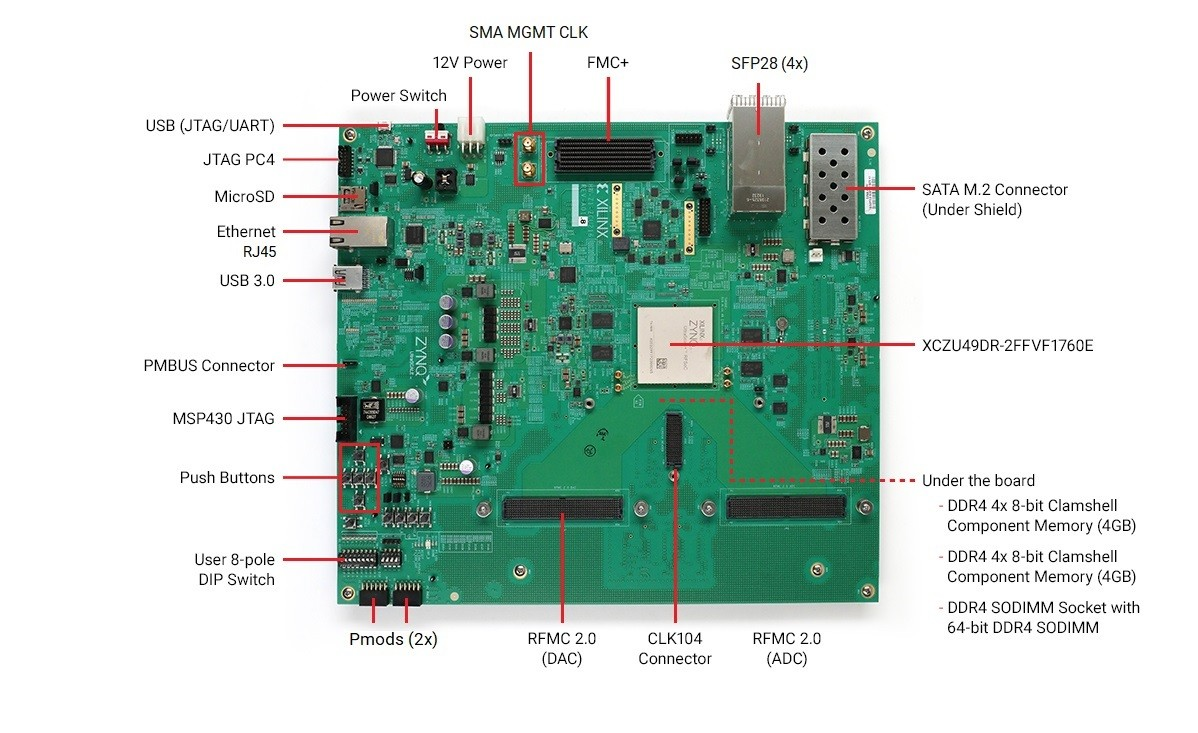
\includegraphics[width = 0.6\textwidth]{chap/05-readout/img/zcu216.png}
%	\caption{Topview of ZCU216 evaluation board with labeled components \cite{zcu216}}
%	\label{fig:zcu216}
%\end{figure}

\paragraph{ZU49DR RFSoC}
Together with an UltraScale+ programmable logic, the ZU49DR \gls{rfsoc} integrates an ARM\textregistered Cortex\texttrademark-A53 \gls{ps}.
This \gls{ps} contains a 64-bit quad-core ARM\textregistered Cortex\texttrademark-A53, serving as \gls{apu}, and a dual core ARM Cortex-R5F, serving as \gls{rpu}.
Furthermore, the system integrates \gls{rf} data converters, allowing to use the system for \gls{rf} applications.
At the moment of writing, this is the industry's only single-chip, adaptable radio platform. \cite{zu49}

\autoref{fig:rfsoc} shows the general block diagram of the \gls{rfsoc}.

\begin{figure}[tb]
	\centering
	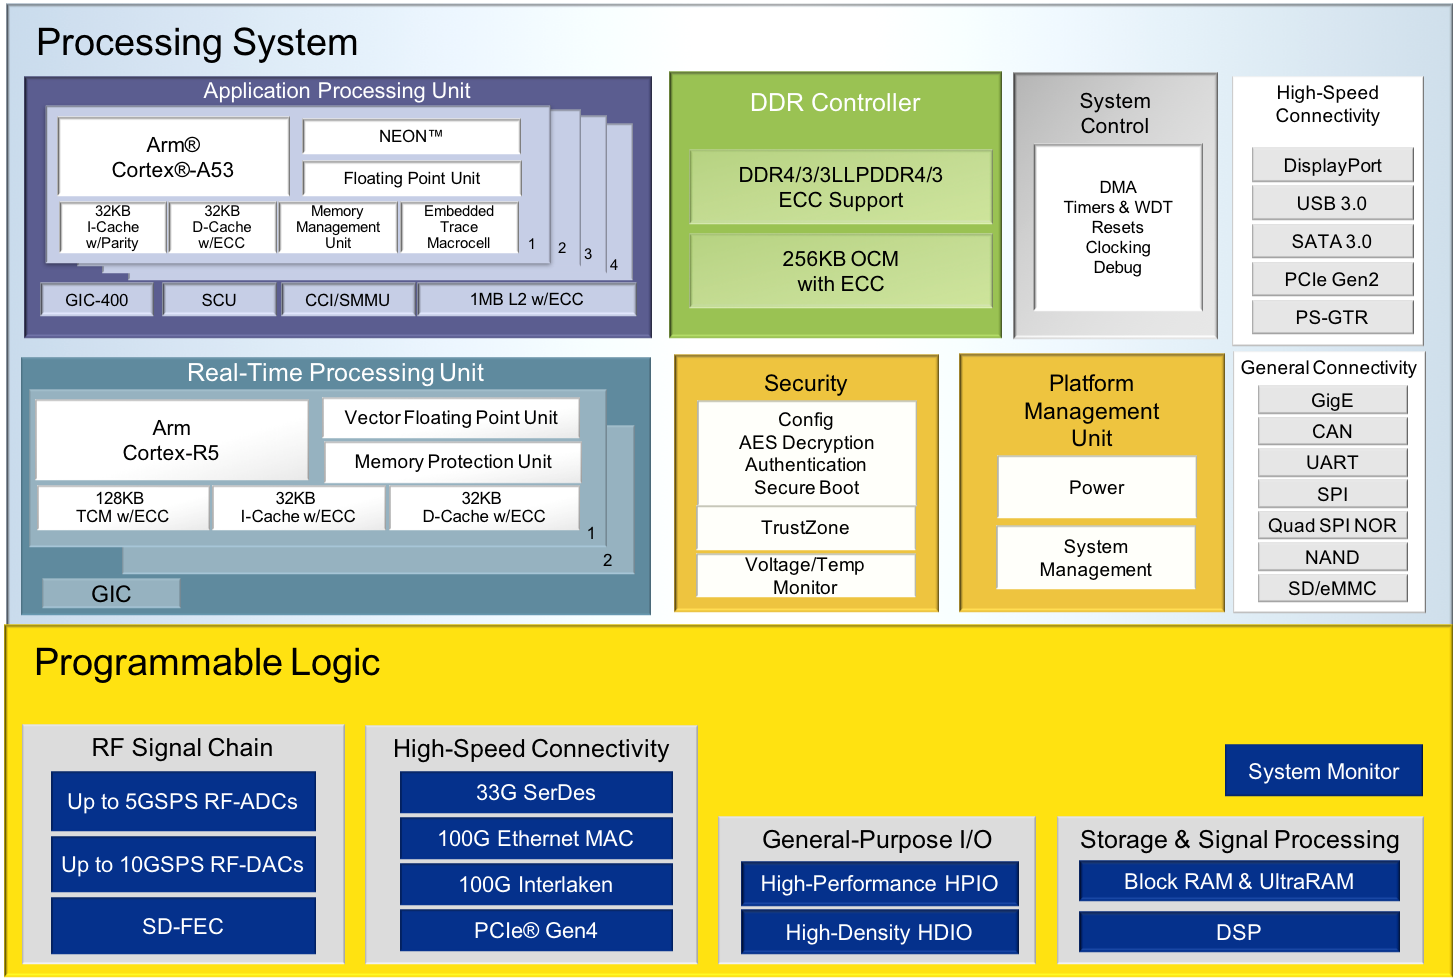
\includegraphics[width = \textwidth]{chap/05-readout/img/rfsoc_blockdiagram}
	\caption[Zynq Ultrascale+ RFSoC block diagram]{Zynq Ultrascale+ RFSoC block diagram, showing in detail the different components of the \gls{ps} and \gls{pl}}
	\label{fig:rfsoc}
\end{figure}


\paragraph{Evaluation Tool}
In order to provide a quick evaluation of data converter performance an evaluation framework from \textit{Xilinx} can be deployed on the card. 
The architecture of the tool is shown in \autoref{fig:evalTool}. \cite{zcu216evaltool}

\begin{figure}[H]
	\centering
	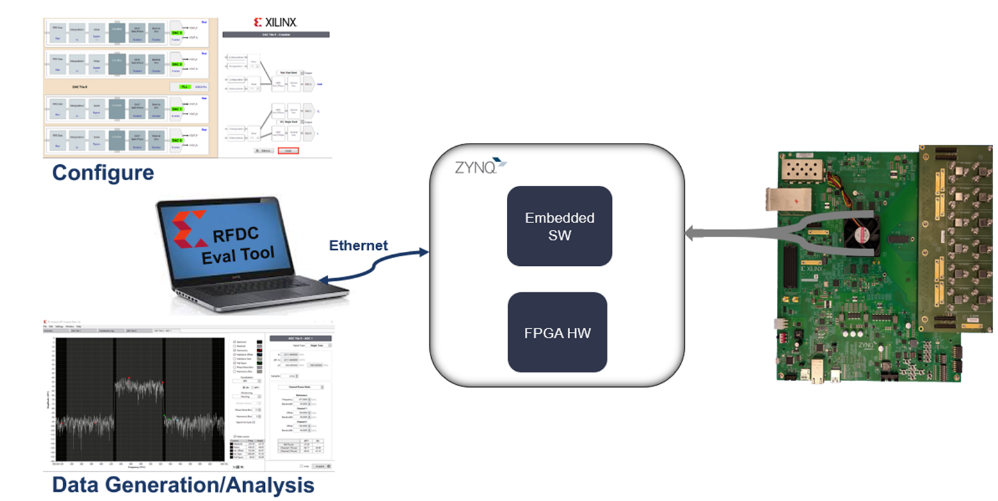
\includegraphics[width = \textwidth]{chap/05-readout/img/zcu216evaltool}
	\caption[ZCU216 Evaluation Tool]{Concept of the Evaluation Tool for the ZCU216, showing the interactions between the host PC and the board \cite{zcu216evaltool}}
	\label{fig:evalTool}
\end{figure}

It enables control of the ZCU216 \gls{ip} cores and the associated designs from a host PC. 
With the tool, different \gls{rf} configurations can be explored, \gls{rf} data can be generated and captured and different \gls{rf} metrics (see \autoref{ssec:adc_charac}) can be observed.  \cite{zcu216evaltool}
For this, the breakout card provided with the board, or any other user-designed board, needs to be attached to the evaluation card via the RFMC connectors\footnote{\gls{fmc} connector for \gls{rf} signals}.

The RF DC (Data Converter) Evaluation Tool consists of two parts:
\begin{itemize}
	\item Hardware design on the \gls{pl}/\gls{fpga}, in order to implement the configuration and data generation/capture of the data converters.
	It is built around the RF Data Converter \gls{ip} Core from Xilinx, descrived in \autoref{sec:firmware}.
	\item Software design on the \gls{ps} and host PC, in order to control the hardware implemented on the \gls{fpga}.
	On the \gls{ps} a Linux application receives commands from the host PC \gls{gui} over Ethernet.
	Based on the commands, it performs the according action, e.g. setting the sampling clock or enabling/disabling data converter channels.
	The \gls{gui} provides a convenient possibility to configure the data converters.
	Data generation via \glspl{dac} can be started, as well as data capture with the \glspl{adc}.
	Furthermore, the tool provides methods to quickly characterize the performance of the data converters (see \autoref{fig:gui}) from which the performance of the plugged break-out board can be derived.
\end{itemize}


\begin{figure}[tb]
	\centering
	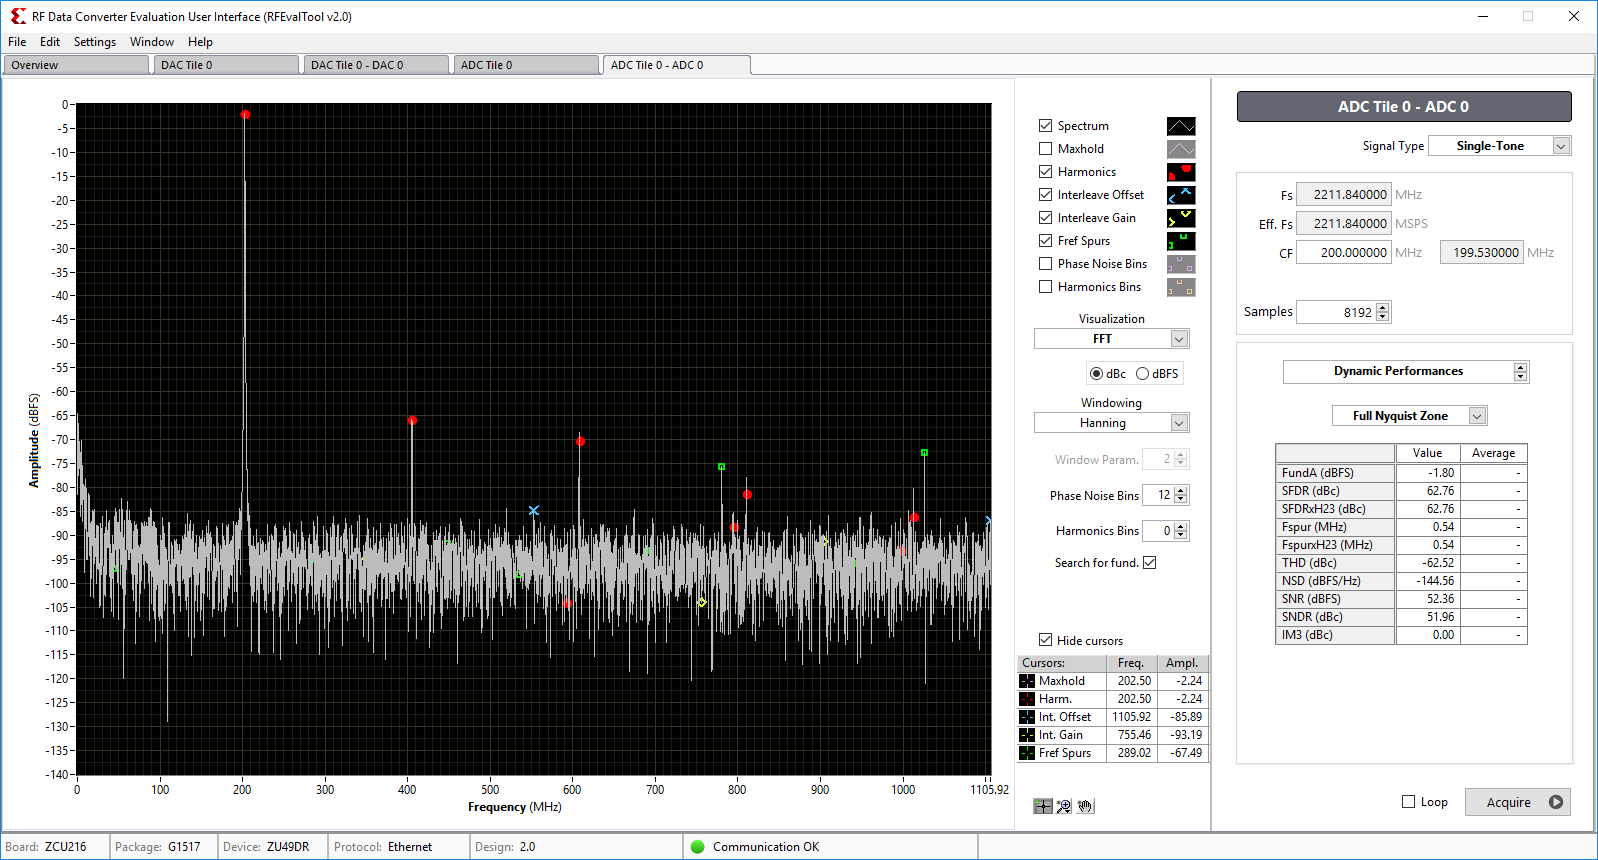
\includegraphics[width = \textwidth]{chap/05-readout/img/evaltool}
	\caption{\gls{gui} of the RF Data Converter Evaluation Tool}
	\label{fig:gui}
\end{figure}

\section{Firmware}\label{sec:firmware}
Similar to the evaluation tool, the firmware for the readout system should contain a software part on the \gls{ps} which allows for control and configuration of the data converters. 
The hardware design part should implement the interface to the sampling board. 
This means it should provide the necessary interfaces to configure the data converters on the readout card, as well as slow control to the delay chips and \glspl{pll} on the sampling board (i.e. through \gls{sdi} and \gls{spi}). 
Furthermore, the high-speed data-throughput interface should be implemented.

\autoref{fig:firmware} shows the general schematic of the firmware on the readout card.
\begin{figure}[tb]
	\centering
	\includegraphics[width = \textwidth]{chap/05-readout/img/firmware.tikz}
	\caption{Schematic of the firmware and processing unit on the readout card}
	\label{fig:firmware}
\end{figure}

The sampled data is propagated from the sampling card to the \glspl{adc} inside the \gls{fpga}. 
This data is written in the \gls{ddr}, from which it is accessible by the data interface, which is responsible for the high-speed data transfer to the following processing node in the \gls{daq} system.
A built-in test-loop is implemented with an integrated \gls{dac}, in order to produce test signals which are propagated to the sampling board.
Configuration of the data converters is done via the Xilinx ``RF Data Converter'' which is described below. 

Components on the sampling board, such as the delay chips, are controlled via \gls{spi} interface. 
This interface is connected to a user bank register, where the user can specify e.g. the desired delay values.

The \gls{ps} communicates with the \gls{pl} via \gls{axi}.
\gls{axi} is a parallel, synchronous, multi-master, multi-slave communication interface.
On the \gls{ps} an operating system, e.g. Linux, or a standalone C application, can run implementing functionalities for the user to be able to control the overall system.
Access to the \gls{ps} is provided by for example via Ethernet or \gls{usb}.


\subsection{Programmable Logic - Hardware design}
For synthesis and analysis of the \gls{hdl} design for the \gls{pl}, the \gls{ide} \textit{Xilinx Vivado} \gls{ide} is used.
To configure and control the data converters, the \gls{rf} Data Converter \gls{ip} Core from Xilinx is used.
In order to program the components on the sampling board, appropriate \gls{spi} interfaces are implemented, respecting the recommendations in the data sheet.

\subsubsection*{RF Data Converter IP Core}
In order to configure the data converters, the \gls{hdl} design should be based around the Xilinx \gls{rf} Data Converter \gls{ip} Core. 
The \gls{ip} core provides a configuration screen, which is used to 
\begin{itemize}
	\item enable the data converter tiles
	\item configure decimation, interpolation and mixing 
	\item set up the sampling rates, \gls{pl} word widths and data types
	\item enable optional interface ports.
\end{itemize}
Handling of the configuration and power-up of the data converters is covered by the \gls{ip} core. 

\begin{figure}[tb]
	\centering
	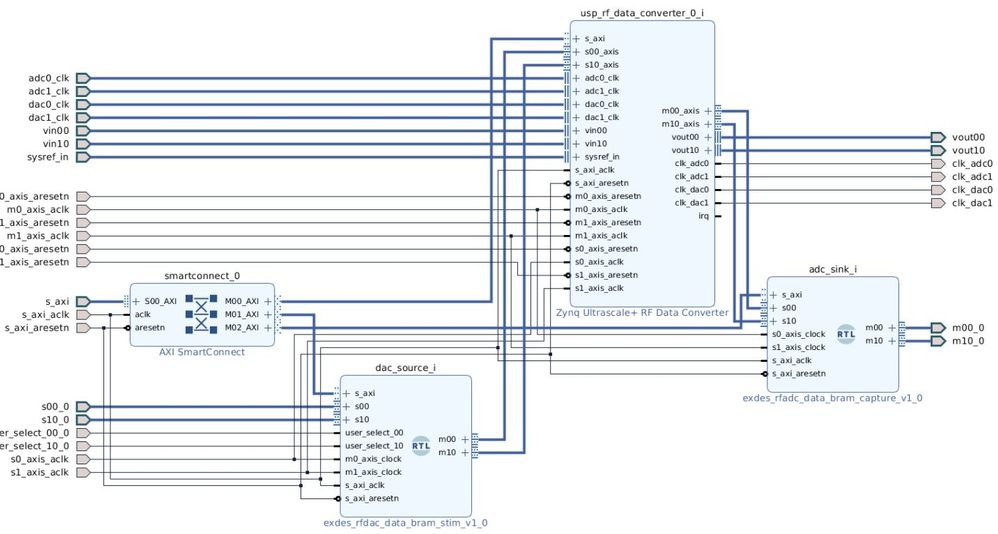
\includegraphics[width = \textwidth]{chap/05-readout/img/rf_data_converter}
	\caption{Simple example design with the \gls{rf} Data Converter}
	\label{fig:rf_dc_ex}
\end{figure}

\subsubsection*{Slow Control}
Components on the sampling board are controlled via a slow control interface. 
As example, the on-bard delay chips are controlled via a \gls{sdi} interface, consisting of four signals: \texttt{EN}, \texttt{SDIN}, \texttt{SCLK} and \texttt{SLOAD}. 
In order to program a certain delay, the timing diagram shown in \autoref{fig:delay_diagram} has to be respected.
The delay chip only accepts data when the EN input is HIGH. 
Therefore, this signal has to remain high in the course of the whole data transaction. 
The data pin, \texttt{SDIN}, which is clocked in by the \texttt{SCLK} signal, has to respect the following structure: delay channel select bit, mode select bit, followed by 9 data bits, which represent the desired delay value in binary format.
At the end, \texttt{SLOAD} has to be asserted HIGH, in order to signal the chip to load the received data into the chip's internal register.
The \gls{hdl} implementation for this interface is listed in \autoref{app:code}. %todo use ref

\begin{figure}[tb]
	\centering
	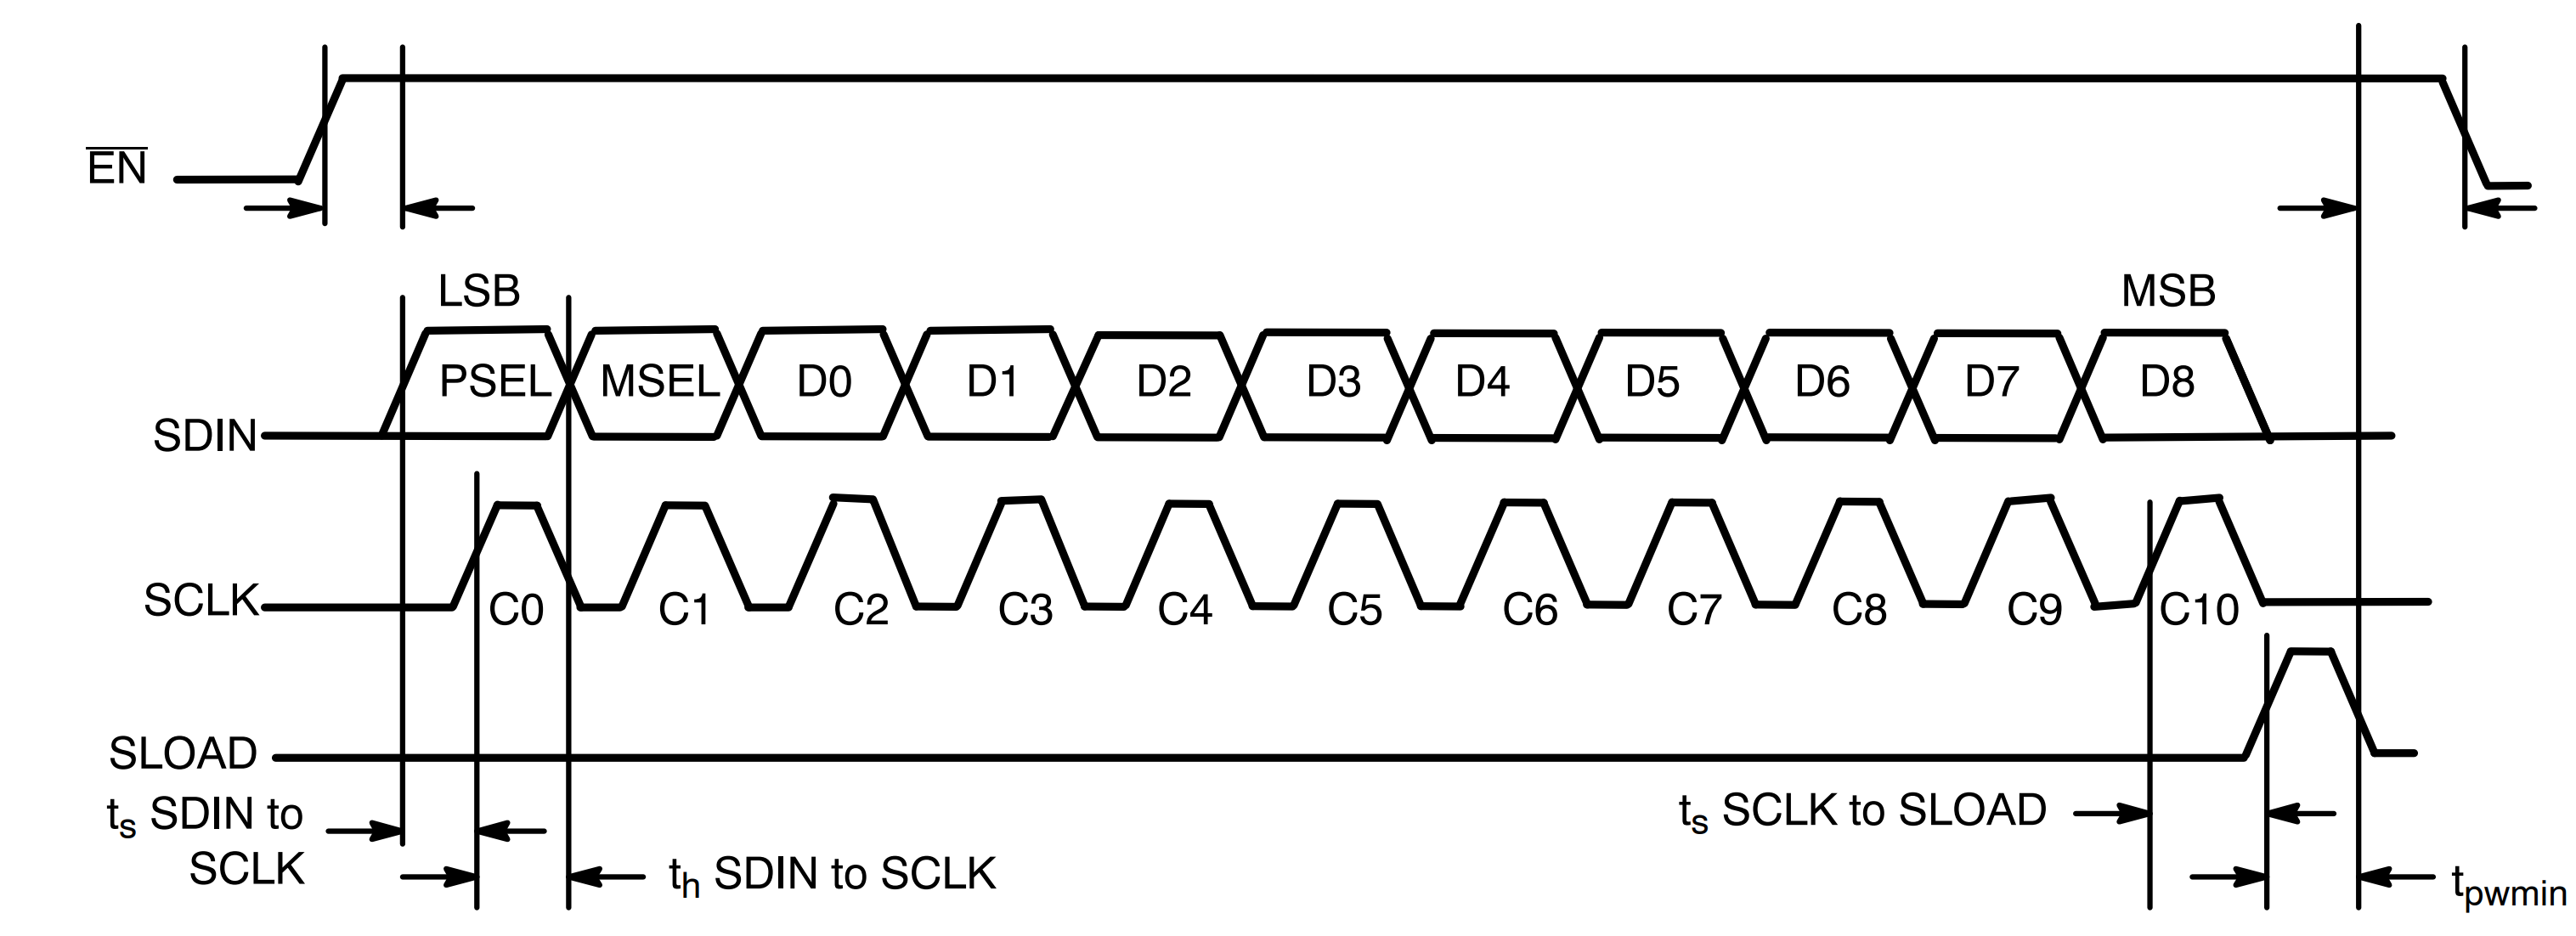
\includegraphics[width = \textwidth]{chap/05-readout/img/sdi_interface_delay}
	\caption{\gls{sdi} timing diagram for the NB6L295 delay chip \cite{NB6L295}}
	\label{fig:delay_diagram}
\end{figure}

In a similar way, the interface for other components is to be implemented.

\subsubsection*{RDMA over Converged Ethernet (RoCE)}
The high speed data interface is implemented using the \gls{roce}.

\Gls{rdma} allows direct memory access from one computer to another over an Ethernet network. This permits high-throughput, low-latency communication between applications which are hosted on clusters of servers or storage arrays. 

\Gls{roce} is a network protocol defined in the \gls{ibta} standard, allowing \gls{rdma} over converged Ethernet network. 
It allows devices to perform direct memory access between each other without involving the host \gls{cpu}. 
The transport processing and memory translation are performed by hardware. 
\Gls{roce} has the benefits of the \gls{rdma} technology and the ease of use and availability of Ethernet.

The ERNIC (Xilinx Embedded RDMA enabled NIC) \gls{ip} provides an Initiator and Target  implementation of \gls{rocev2} enabled \gls{nic} functionality. This \gls{ip} is specifically designed for embedded applications that require reliable transmission over Ethernet networks.

\autoref{fig:ernic} shows a possible working principle of a system with multiple host CPUs and multiple native \gls{nvme}\footnote{ \gls{nvme} is an open, logical-device interface specification for accessing a computer's non-volatile storage} devices talking over a network fabric through the Xilinx \gls{ernic} \gls{ip}
subsystem.

\begin{figure}[H]
	\centering
	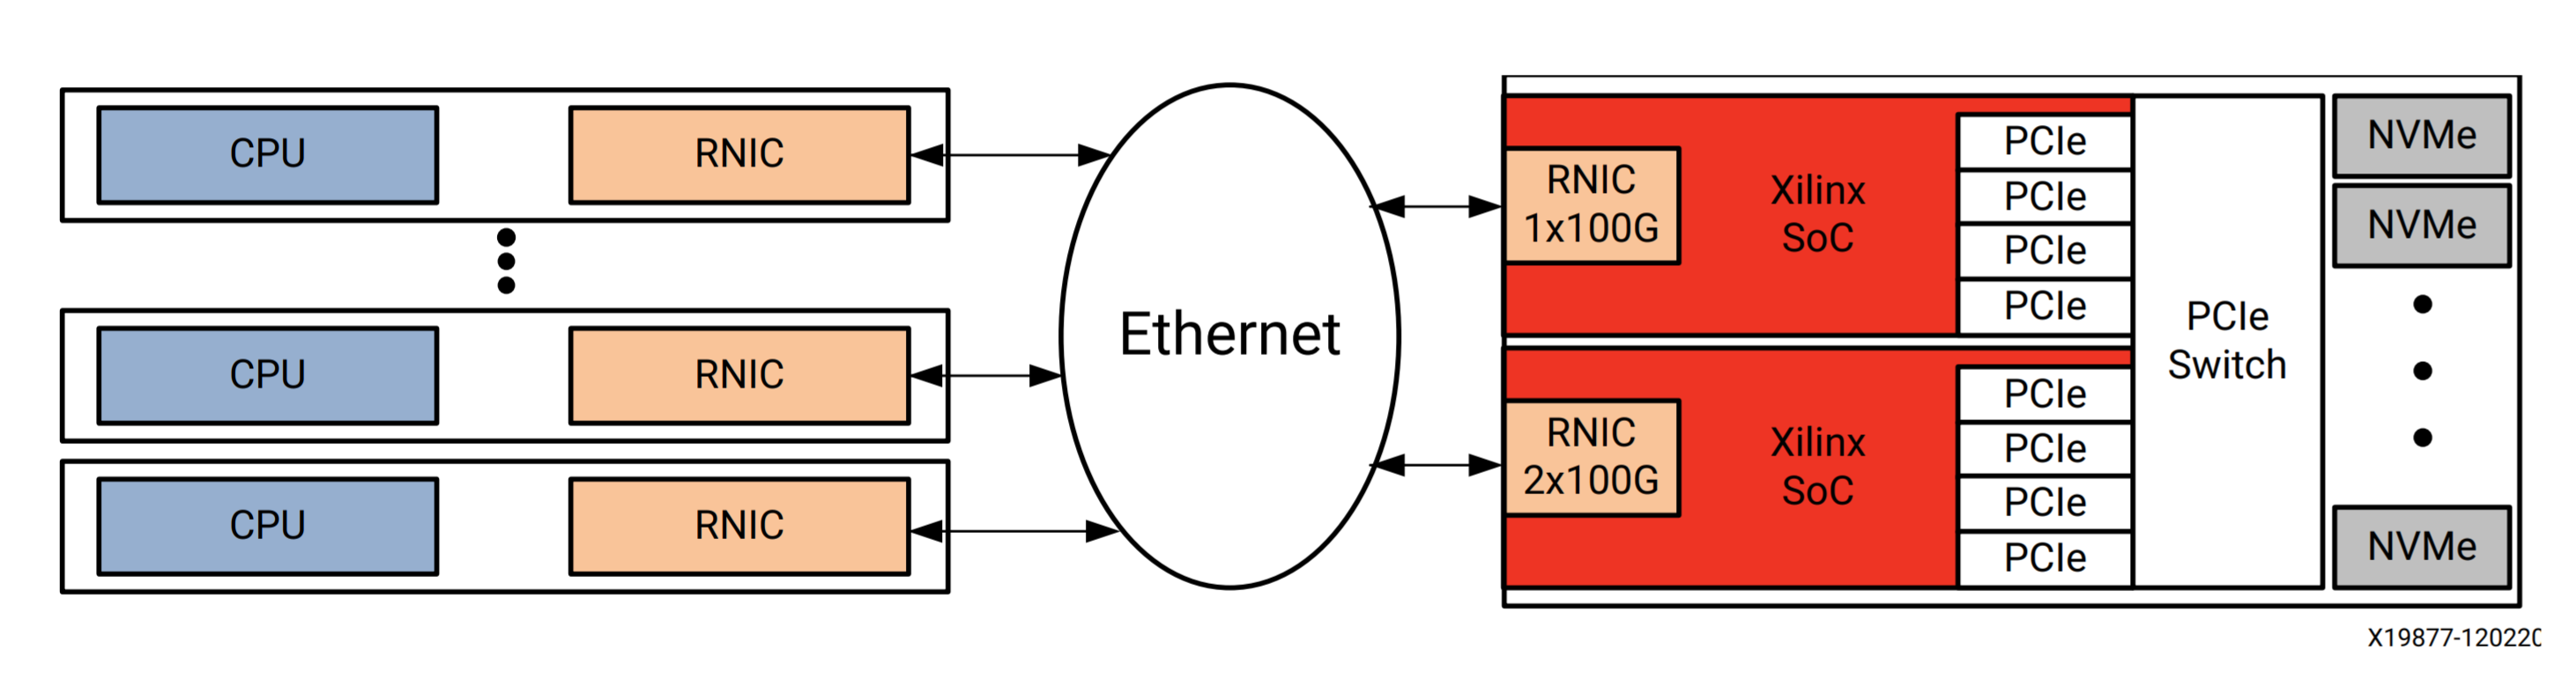
\includegraphics[width = \textwidth]{chap/05-readout/img/ernic}
	\caption{Xilinx ERNIC working principle example}
	\label{fig:ernic}
\end{figure}

\subsection{Processing Unit - Software Design}
In order for the user to be able to control the whole system, some kind of application has to be implemented for control of the hardware design.
For this the \gls{ps} side of the \gls{rfsoc} is used. 
The ARM Cortex processor allows to implement standalone C application, as well es hosting an operating system like Linux. 
Providing a number of peripheral connections, like Ethernet or \gls{usb}, the \gls{ps} can easily be accessed by the user from another host computer, given the necessary drivers and protocols are implemented. %todo RJ-45 is a bit dangerous (the real name is 8P8C or 8P4C). better say ethernet
The aforementioned evaluation tool for example uses the Linux application \textit{rftool} in order to receive commands and perform the according action.

For interaction and monitoring of the data converters the RFdc driver \gls{api} needs to be used.
It is available both as bare-metal and Linux driver and includes functionalities to respond to interrupt, change settings (e.g. mixer frequency of the data converters) and interaction woth the RF Data Converter \gls{ip}

In order to implement and build software applications, the novel \textit{Xilinx Vitis} unified software platform is used.
It enables the development of embedded software and accelerated applications on heterogeneous \textit{Xilinx} platforms including \glspl{fpga} and \glspl{soc}.
It offers \glspl{api} and libraries for accelerated development of software applications for the system under development.
The applications can be programmed with common languages like C, C++, and Python.
